\chapter{Team 1 Agent Design}\label{team_1_agent_design}

\section{Overview}

The following chapter presents the design and implementation of Team 1's agent. The agent presented agent seeks to imitate important parts of human behaviour such as social status, social networks, selfishness, forgiveness and learning from experiences. At the end of the chapter, it will be shown that by using these concepts, the agent produces better collective outcomes over agents performing random actions.

\section{Core Structure}
Figure \ref{fig:agent_structure} presents a high-level overview of the structure and operation of our agent. In broad terms, the agent contains three elements which impact decision-making. These elements are:
\begin{enumerate}
  \item Social capital: Socially constructed resources which facilitate cooperation to solve collective problems.
  \item Selfishness: A continuously updated variable dictating to what degree an  agent prioritizes its own utility over the social welfare of the group when making decisions. 
  \item Q-functions: Functions learned through reinforcement learning which estimate the impact of actions given the current game state.
\end{enumerate}
In addition to these components which are inherent to the agent, the current state of the game, known as the \emph{environment}, also influences decisions. Exactly how each component is used in the decision making process varies between different types of decisions, and social capital, selfishness and q-functions are not all used for every decision. The specific decision process for each type of decision will be discussed in greater detail in \ref{}.

%However, a general decision flow can be as follows: The agent takes in the current game state and passes it through a set of Q-functions. The Q-functions return the expected utility of each action to the collective and to the agent itself. Based on its current selfishness value, the agent aggregates the two utility values into a single value for each action.   Generally, the decision flow 

After each round of the game, the agents will update their internal state. Specifically, the agents will update their selfishness based on the current environment and the social capital of agents, while the social capital will be updated based on the actions of agents. The social capital is also updated every time an agent receives a message from an agent in their network. All of these update mechanisms are indicated by red arrows in Figure \ref{fig:agent_structure}. As can be seen, there is no arrow feeding back to the Q-functions as they do not update over the course of a single game. Instead, the Q-functions are updated based on the results from a series of games. However, as will be discussed later, the updating of selfishness values does still permit the agents to learn from experiences during a game.

\begin{figure}[!h]
    \centering
    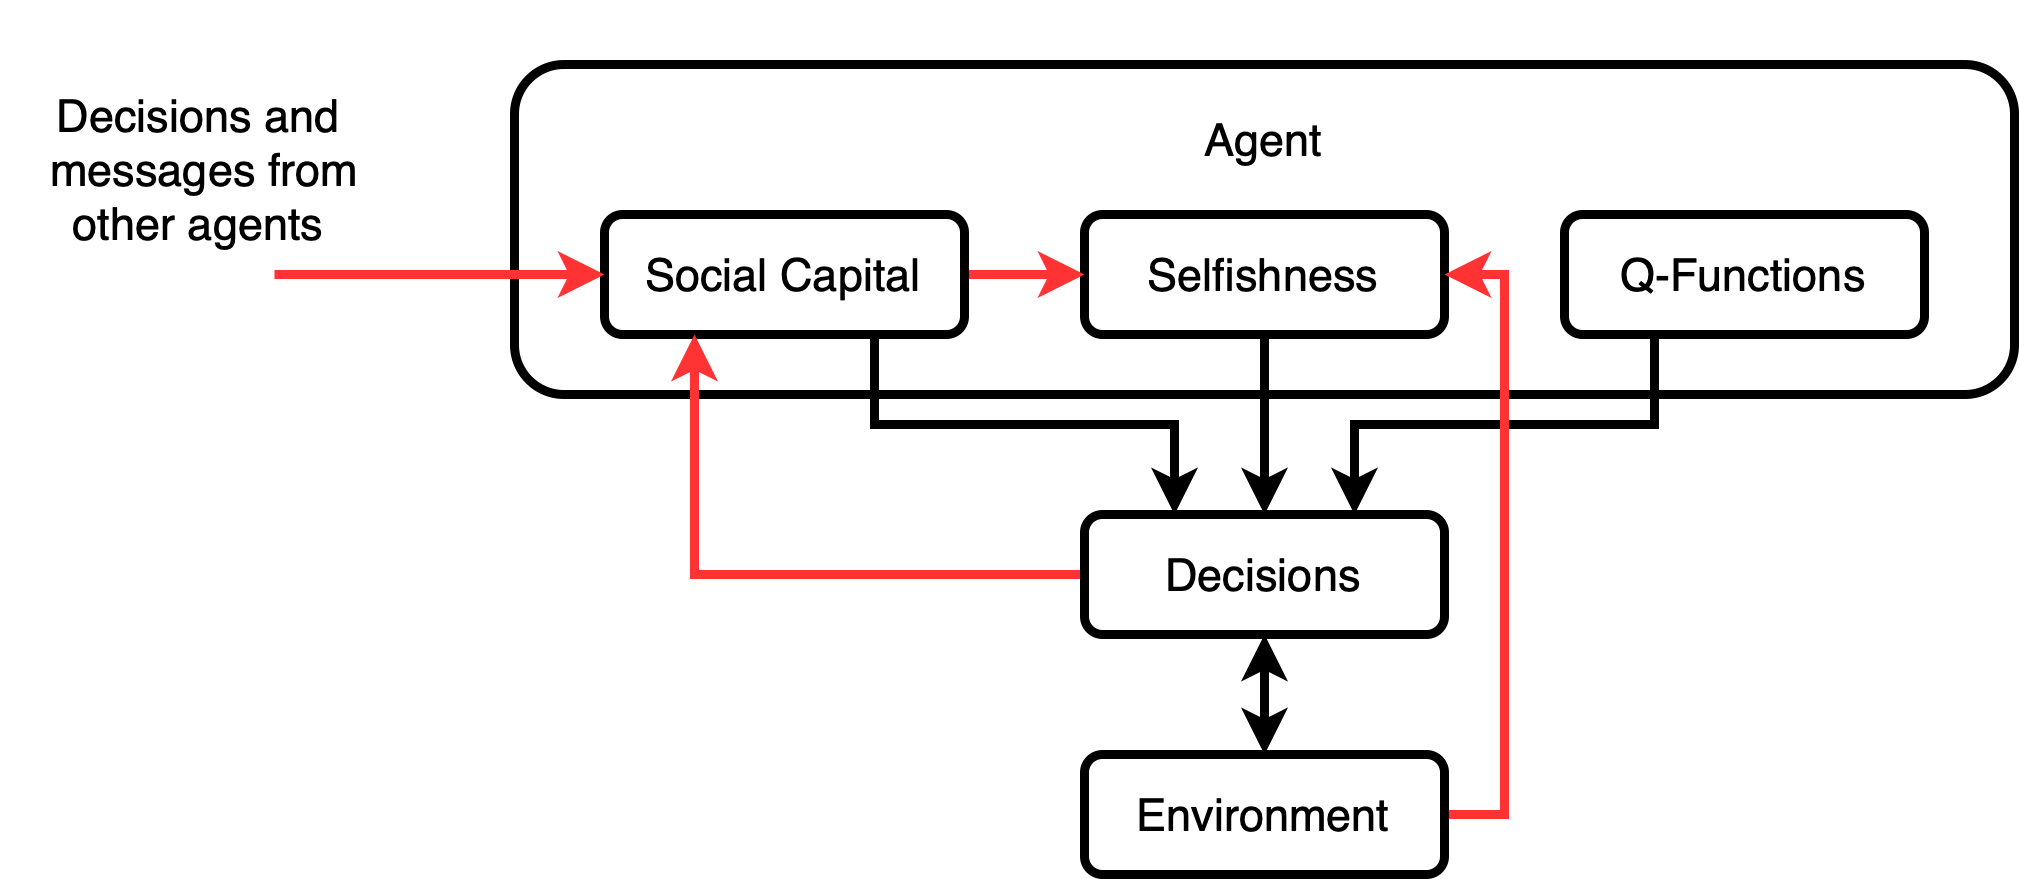
\includegraphics[width=0.75\linewidth]{004_team_1_agent_design/images/agent_structure.png}
    \caption{Overview of agent structure.}
    \label{fig:agent_structure}
\end{figure}

\section{Social Capital}

The core concept underlying the design of the agent is the idea of social capital. The exact definition of the term "social capital" varies between works, but can be summarized as "an 'umbrella term' for a range of socially constructed conceptual resources that help people coordinate expectations and self-organise."\cite{pitt}. Several forms of social capital have been identified and defined. Our work on social capital is mostly related to those forms laid out by Elinor Ostrom and T. K. Ahn in their 2007 paper "The meaning of social capital and its link to collective action". \cite{ostrom-ahn} In their paper, Ostrom and Ahn identified three forms of social capital. These were \emph{Institutions}, \emph{Networks} and \emph{Trustworthiness}. In addition to the forms of social capital presented by Ostrom and Ahn, we have as a team identified another form of social capital elected to call \emph{Honour}. With \emph{Honour} we refer to the human tendency to want to return a favour, or similarly, our appetite for revenge. A more comprehensive definition of honour is given in section \ref{subsection:honour}. 


In order to use social capital to promote cooperation, it must be used as part of a framework where the actions of an agent impact their social capital and where the social capital is used to make informed decision on whether or not to cooperate with other agents. For our agent, we used a similar framework to that presented by Petruzzi, Pitt, and Busquets\cite{complexity_reduction}. An overview diagram of this framework is presented in Figure \ref{fig:social_capital_framework}.

We did however make modifications to the framework.


Social capital is today an ubiquitous concept within the social sciences, and enables the solving of. 

Various formulations exist for the str. For our agent, we have specifically developed upon the framework for social captial which Elinor Ostrom and T. K. Ahn in their 2007 paper "he meaning of social capital and its link to collective action". \cite{ostrom-ahn} In their paper, Ostrom and Ahn identified three forms of social capital. These were \emph{Institutions}, \emph{Networks} and \emph{Trustworthiness}. In addition to the forms of social capital presented by Ostrom and Ahn, we have as a team identified another form of social capital elected to call \emph{Honour}. A more comprehensive definition of honour is given i section \ref{subsection:honour}. Together, the. 

To keep track of the social capital of other agents, each agent has a map which maps each agent id to an array of 4 values. From index 0 to index 3, this array holds values describing the social capital related to institutions, networks, trustworthiness and honour respectively. Each of these numbers is bounded between -1 and 1, where a higher number indicates higher social capital. These arrays are all initialised with values of 0. This is a neutral state and denotes that the agent currently does not have any opinion about the other agent. If other agents do non-cooperative actions, the array values will decrease and become negative numbers. This indicates that our agent disapproves of the actions of the other agents. Inversely, if another agent performs a cooperative actions, this will cause the array values to increase. This indicates that our agent approves of the actions of the other agent.

Framework of social capital

\begin{figure}[!h]
    \centering
    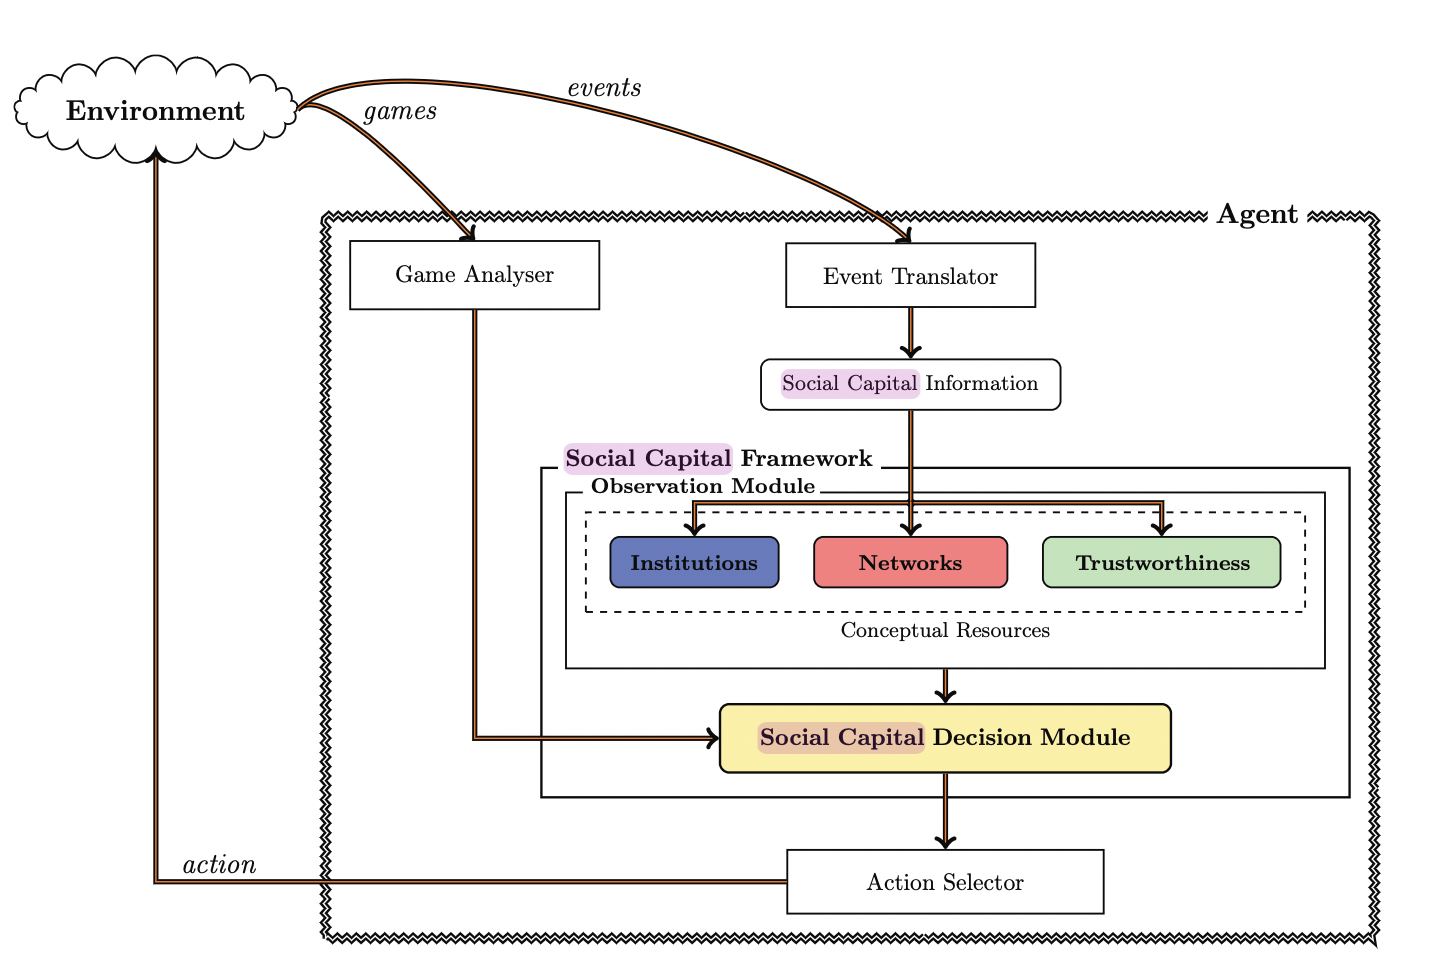
\includegraphics[width=0.75\linewidth]{004_team_1_agent_design/images/socialcapitalframework.png}
    \caption{Framework for a social capital system.\cite{pitt}}
    \label{fig:social_capital_framework}
\end{figure}

\subsection{Institutions}

\subsection{Networks}

\subsection{Trustworthiness}

\subsection{Honour}
\label{subsection:honour}

\section{Forgiveness}

\section{Selfishness}

Starts at a random value, as such we get agents with differing behaviour. Hope is that the social capital framework through sanctions encourages cooperative behaviour and thus low selfishness in the group as a whole.

Weighting of how much agent prioritises its own performance over the performance of the group as a whole.

\subsection{Impact on Decision Making}

\subsection{Updating Selfishness}


\section{Sanctions}

\subsection{Exclusion from Trading}

\subsection{Elections}

\section{Q-learning}

\section{Experiments}
do not use HP-pool as it is OP

\section{Agent Performance}

\section{Conclusion}